\documentclass[journal]{IEEEtran}
\IEEEoverridecommandlockouts
\usepackage{graphics}
\usepackage{rotating}
\usepackage{epsfig}
\usepackage{amsmath}
\usepackage{amssymb}
\usepackage[spanish]{babel}
\usepackage{cite}
\usepackage{hyperref}
\usepackage{float}
\usepackage{csvsimple}
\usepackage[justification=centering]{caption}
\usepackage{atbegshi} % erase first blank page
\AtBeginDocument{\AtBeginShipoutNext{\AtBeginShipoutDiscard}}

% Ajustes de paquetes


\title{\LARGE \bf Ruteo de entrega de productos para una empresa de e-commerce}

\author{Juan Pablo Echeagaray González, Emily Rebeca Méndez Cruz, \\Carolina Longoria Lozano, Verónica Victoria García De la Fuente \\
Optimización determinista \\
MA2001B.200 \\
Dr. Fernando Elizalde Ramírez \\
Dr. Jaime Eduardo Martínez Sánchez}% <-this % stops

\begin{document}

    \thanks{Verónica Victoria García De la Fuente, Emily Rebeca Méndez Cruz, Carolina Longoria Lozano, Juan Pablo Echeagaray González pertencen al Tec de Monterrey Campus Monterrey, N.L. C.P. 64849, Mexico {\tt\small}}

    \maketitle

    \thispagestyle{empty}
    \pagestyle{empty}

    \begin{abstract}
        Una empresa de e-commerce ha solicitado que alumnos del Tecnológico de Monterrey diseñen un programa de rutas para la entrega de los productos adquiridos por sus clientes en su tienda \texttt{online}. Con las bases de datos recibidas se formuló un modelo de CVRP, este modelo fue embebido y optimizado para minimizar las distancias recorridas por los camiones de entrega. El producto final despliega un reporte de las rutas así como una visualización de estas.
    \end{abstract}

    \begin{IEEEkeywords} 
        CVRP, Programación Entera, Metaheurísticos, Open Source Software
    \end{IEEEkeywords}

    \section{Introducción} \label{sec:intro} % Abstract expandido, tiene que incluir como está repartido el escrito

    \section{Contexto general} \label{sec:general-context}
        
    \section{Objeto de estudio} \label{sec:case-study}

        Nuestra implementación se enfoca en resolver el problema de ruteo para la entrega de productos, siendo esto un problema conocido como CVRP (Capacitated Vehicle RoutingProblem); en este se busca encontrar un conjunto de rutas para una flotilla de vehículos que tenga el menor costo de ruta en el que se realicen todas las entregas necesarias. Cada uno de los vehículos de la flotilla sale del mismo centro de distribución, y al final de su ruta debe de regresar a este \cite{elshaer2020taxonomic}.

        Los vehículos solamente realizarán entregas a los clientes de la empresa, es decir, no habrá etapa alguna de carga de paquetes más que en el centro de distribución; aunado a esto, cada uno de los clientes se visitar una sola vez, esto hace referencia a que si uno de los clientes ordenó más de un producto, se entregarán todas sus ordenes en el momento en que sea visitado.
        
        No se toma en cuenta un límite de distancia recorrida por vehículo ni tampoco se consideran ventanas de tiempo para realizar las entregas.
    
    \section{Planteamiento del problema} \label{sec:problem}

        Sean los conjuntos:
        \begin{align*}
            & i \in \{1, \dots, n \} \\
            & j \in \{1, \dots, n \} \\
            & k \in \{1, \dots, V \}
        \end{align*}
        
        Sean los parámetros:
        \begin{align*}
            & V: \text{Número de vehículos disponibles} \\
            & Q: \text{Capacidad de carga máxima del vehículo en } m^3 \\
            & n: \text{Número de clientes a visitar} \\
            & c_{ij}: \text{Distancia geodésica entre el punto } i \text{ y el punto } j \\
            & d_j: \text{Demanda en } m^3 \text{ del cliente } j 
        \end{align*}
        
        Sean las variables:
        \begin{align*}
            & x_{ijk}: \text{Variable binaria que toma el valor de 1}\\
            & \text{si el arco del punto i al punto j} \\
            & \text{forma parte de la ruta óptima recorrida por el vehículo } k \\
            & x_{ijk} \in \{0, 1\}
        \end{align*}
        
        Modelamos el problema de optimización como:
        
        \begin{equation*}
            \begin{aligned}
                \text{min } \quad & z = \sum_{k=1}^{V} \sum_{j=1}^{n} \sum_{i=1}^{n} c_{ij} x_{ijk}\\
                \text{sujeto a: }\quad &
                \begin{array}{c}
                    \displaystyle\sum_{i=1}^{n} x_{ijk} = \sum_{i=1}^{n} x_{jik} \\[3pt]
                    \displaystyle\sum_{k=1}^{V} \sum_{i=1}^{n} x_{ijk} = 1 \\[3pt]
                    \displaystyle\sum_{j=2}^{n} x_{1jk} = 1 \\[3pt]
                    \displaystyle\sum_{i=1}^{n} \sum_{j=2}^{n} d_{j} x_{ijk} \leq Q \\[3pt]
                    u_{j} - u_{i} \geq d_j - Q (1 - x_{ijk}) \\[3pt]
                    d_i \leq u_i \leq Q \\[3pt]
                    x_{ijk} \in \{0, 1\}
                \end{array}
            \end{aligned}
        \end{equation*}
        
        Las restricciones anteriores hacen referencia a:
        \begin{enumerate}
            \item Número de veces que un camión entra por un punto debe de ser igual que el número de veces que las que sale
            \item Cada camión solamente puede entrar 1 vez a un punto
            \item Todos los vehículos salen del CEDIS
            \item Límite a la capacidad de carga máxima del vehículo
            \item Las últimas 2 restricciones eliminan los \emph{sub-tours}
        \end{enumerate}
        
        Para la problemática actual, estamos planeando realizar 192 entregas ($n$), se dispondrán de 9 vehículos $(V)$, cada uno de ellos tendrá una capacidad máxima de carga de 18 $m^3$ ($Q$). Los valores numéricos para las demandas y distancias son calculados dentro de la aplicación.
        
        El heurístico que usamos en nuestro modelo es el costo asociado de ir de un punto de la ciudad a otro, en nuestro modelo la distancia entre 2 puntos de entrega funge ese papel. No estamos modelando la distancia que hay entre cada punto como la distancia manejando, sino que estamos usando la distancia geodésica que hay entre cada punto, una de las principales virtudes de este heurístico es la sencillez con la que puede ser calculado y tampoco se requiere requerir a software comercial para obtenerse. 
        
        Hemos decidido seguir adelante con este heurístico ya que hay varios proyectos reconocidos que lo usan para resolver problemas de ruteo de vehículos \cite{ERDOGAN201762}.

    \section{Justificación} \label{sec:justification}

        Actualmente el e-commerce a crecido un 55\% debido a la pandemia y la tendencia es que se mantenga el número de ventas actual \cite{koetsier-2022}, siendo esto un reto para la logística de entrega, la cual afecta directamente al precio de venta, por lo tanto en los gastos de la empresa viendo reducidas sus utilidades, de ahí la necesidad del desarrollo de nuestro proyecto ya que consistes en generar soluciones de forma rápida a este tipo de problemas beneficiando a la empresa y al cliente, ya que se eficientiza el proceso, se optimizan los recursos y mejora la calidad de servicio hacia el cliente

    \section{Marco teórico} \label{sec:theoretical}
    
        El \emph{Traveling Salesman Problem}, conocido como \emph{Problema del Agente Viajero} en español, es un problema que se encarga de buscar la ruta más corta y eficiente para llegar a un destino. Esta se basa en que existen múltiples opciones de llegar a un mismo destino, pero enfocándose en reducir costos de transporte, por lo que obtenemos de solución la ruta más corta \cite{trevelingProb}.

        Para ésta problemática se tiene contemplado que entre más destinos haya automáticamente el nivel de complejidad para el cálculo de la solución óptima aumenta. Por esta razón TSP es clasificado como un problema de NP-Hard, de acuerdo con la teoría de la complejidad computacional \cite{trevelingProb}.

        Para la solución de este problema existen diferentes métodos debido a la popularidad y complejidad que tiene, estos son algunos de ellos:
        
        \subsection{Vecino más cercano}
        
            También conocido como KNN, este es uno de los algoritmos más simples para resolver este problema. Se trata de un método de aprendizaje automático básico aplicado para la logística de transporte, en este caso, el conductor -o agente viajero- siempre comienza su recorrido con el destino más cercano. Aunque para este método la solución encontrada no siempre logra la optimización \cite{trevelingProb}.

        \subsection{Ramificación y atadura}
        
            El método Branch and Bound es un algoritmo complejo diseñado para solucionar problemas que cuentan con variables de decisión enteras; para este método, el problema se divide en múltiples sub-problemas donde cada uno de estos tiene varias soluciones posibles. Se debe destacar que al seleccionar una solución, esta puede afectar en las posibles soluciones de sub-problemas posteriores, ya que como su nombre lo indica, actúa de manera ramificada. Este método se aplica como solución del problema del vendedor viajero \cite{trevelingProb}.

        \subsection{Fuerza bruta}
        
            Consiste en la enumeración sistemática de todas las posibles rutas de distribución, se calcula y compara todas las posibles soluciones revisando cuál o cuáles de ellas cumplen mejor a los objetivos de la empresa. Esto con el fin de establecer una única solución, que para el caso de este problema, sería la más corta y por ende la óptima \cite{trevelingProb}.
    
    \section{Objetivos} \label{sec:objectives}

        El objetivo principal de nuestro trabajo es generar una metodología para resolver el problema de generación de rutas de entrega para una empresa de e-commerce que se acerque a la optimalidad. De forma específica, se desea encontrar un conjunto de $n$ rutas que realicen todas las entregas de 1 día para la empresa, estas rutas deben de minimizar la distancia total recorrida así como respetar las diversas restricciones propias del problema y de la empresa

    \section{Hipótesis} \label{sec:hyp}
            
        Proponemos una implementación que es capaz de obtener resultados cercanos a la solución óptima en tiempos aceptables, con un costo computacional bajo, en relación a otras implementaciones. 
    
    \section{Metodología} \label{sec:method}

        Se realizará una limpieza de las bases de datos proporcionadas por medio de un lenguaje de programación; con estas se determinarán las entregas a hacer en 1 día y se obtendrán los domicilios de los clientes, estos serán después geo-codificados para calcular una matriz de distancias todos contra todos.

        En conjunto con la matriz de distancias y el volumen de los pedidos de cada cliente se realizará un proceso de optimización con un \texttt{solver} de libre distribución. Finalmente se desplegará un reporte con el conjunto de rutas encontradas en un mapa en adición a datos generales de la solución propuesta, tales como el volumen muerto y el consumo de gasolina.

    \section{Propuesta metodológica} \label{sec:prop-method}
    
        Para la solución de esta problemática hemos usado el lenguaje de programación Python; para los procesos de lectura, limpieza, exploración y agregación de datos hemos usado la librería \texttt{pandas} en conjunto con \texttt{matplotlib} y \texttt{seaborn}, para la solución del problema de programación lineal usamos la librería \texttt{ortools} de Google, y para la visualización de los rutas generadas hemos usado \texttt{folium}. Una liga al código fuente que hemos desarrollado se encuentra en el apéndice \ref{code:repo}.
        
        \subsection{Limpieza de la base de datos} \label{stage 1}
            
            Hemos recibido 4 bases de datos. Una conteniendo las direcciones de los centros de distribución de la empresa, un archivo que contiene un listado de todos los productos que vende más algunas de sus propiedades, en particular nos interesa el volumen de cada artículo. Disponemos también de un archivo que contiene todos los tipos de vehículos que la empresa usa para realizar las entregas, y una base de datos que contiene un listado de las entregas que se deben de realizar.
            
        \subsection{Procesamiento de domicilios} \label{stage 2}
        
            Para la geo-codificación de los domicilios hemos usado la librería \texttt{Photon}, desde el paso anterior hemos creado una columna que contiene todos los datos de referencias de los domicilios de los compradores. El proceso de geo-codificación toma un tiempo promedio de 15 minutos en la máquina que usamos, en promedio se logran codificar 25\% de los domicilios que recibe. Al final de este proceso tenemos las coordenadas asociadas a cada uno de los domicilios.

        \subsection{Cálculo de matriz de distancias} \label{stage 3}
            
            De las coordenadas de cada domicilio calculamos una matriz de distancia todos contra todos, la distancia a usar es la geodésica. Como función geodésica hemos usada la implementada en el módulo \texttt{distance} de la librería \texttt{Geopy} usada para el procesamiento de domicilio, y la matriz de distancia se calcula con la misma a través de la función \texttt{cdist} implementada en el sub-módulo \texttt{spatial} de la librería de cómputo científico \texttt{SciPy}.

        \subsection{Generación de rutas} \label{stage 4}
        
            Para la solución del problema hemos usado la librería \texttt{ortools} de Google. Hacemos uso de la matriz de distancias calculada en el paso anterior, un listado de cuánto volumen debe de ser entregado a cada uno de los clientes, un número de vehículos a mandar, y su capacidad máxima de carga en metros cúbicos. La solución generada consiste de un listado de las rutas a seguir por cada uno de los vehículos, el volumen total que llevarán, cuál fue la distancia total recorrida por todos los vehículos y cuánta carga llevaron.

        \subsection{Visualización de rutas} 
            
            La visualización de rutas se realizó con la API de la librería \texttt{folium}, con ella hemos generado un mapa de Monterrey en la que se visualizan las rutas que siguen todos los vehículos; el mapa también despliega información del domicilio al que se realiza la entrega, y el volumen total de los productos que debe de recibir.
        
        \subsection{Resumen de resultados}

            Del resultado de generación de rutas se despliega también un tabulado en el que se concentran métricas para cada uno de los vehículos de la flotilla, el tabulado contiene información como:
            \begin{enumerate}
                \item Número de clientes visitados
                \item Distancia total recorrida en $km$
                \item Carga del vehículo en $m^{3}$
                \item Volumen muerto en $m^{3}$
                \item Gasolina consumida en $l$
            \end{enumerate}

            Dada la instancia de VRP que intentamos resolver, suponemos que la flotilla es homogénea; es decir, todos los vehículos tienen la misma capacidad de carga y tienen el mismo rendimiento de combustible. Es por esto que podemos calcular un consumo de gasolina y una huella de carbono.
            
    \section{Experimentación y resultados} \label{sec:experimentation}
    
        La red con la que tratamos consta de 193 nodos, 192 referentes a los clientes, y 1 nodo más para el Centro de Distribución. El número de conexiones (aristas) dentro del grafo es $193\choose2$ = $18528$
        
        Dada la complejidad computacional de resolver de forma exacta un VRP con 193 nodos, deben de utilizarse heurísticos en el proceso de solución. La librería \texttt{ortools} le permite al usuario seleccionar 1 heurístico para la obtención de una solución inicial a mejorar, y 1 meta-heurístico para realizar el proceso de optimización. Es también decisión del desarrollador imponer un límite al tiempo de ejecución del que dispone el algoritmo, este parámetro también deberá ser optimizado en base a los resultados generados.

        Para obtener una solución básica inicial hemos optado por utilizar un algoritmo de naturaleza voraz que selecciona como siguiente nodo a visitar a aquel con el menor costo de ruta asociado; este proceso se repite para cada uno de los vehículos de la flotilla. Como metaheurístico hemos seleccionado una búsqueda local guiada, que de acuerdo a la documentación de la librería \cite{google-2021} suele ser la mejor opción para resolver problemas de ruteo de vehículos.

        \subsection{Ajuste de parámetros} \label{sec:parameter-tuning}
            
            Para determinar cuál es el mejor tiempo límite se obtuvieron 10 muestras de resultados para tiempos máximos de cómputo de entre 1 y 10 segundos. Se recuperó la mejor distancia encontrada, así como la media, el máximo, la desviación estándar y la varianza. En la figura \ref{fig:optim-curves} se presentan las curvas de optimización generadas, se grafica la distancia mínima encontrada, la distancia media y la máxima del conjunto de 10 muestras.
            \begin{figure}[h!]
                \centering
                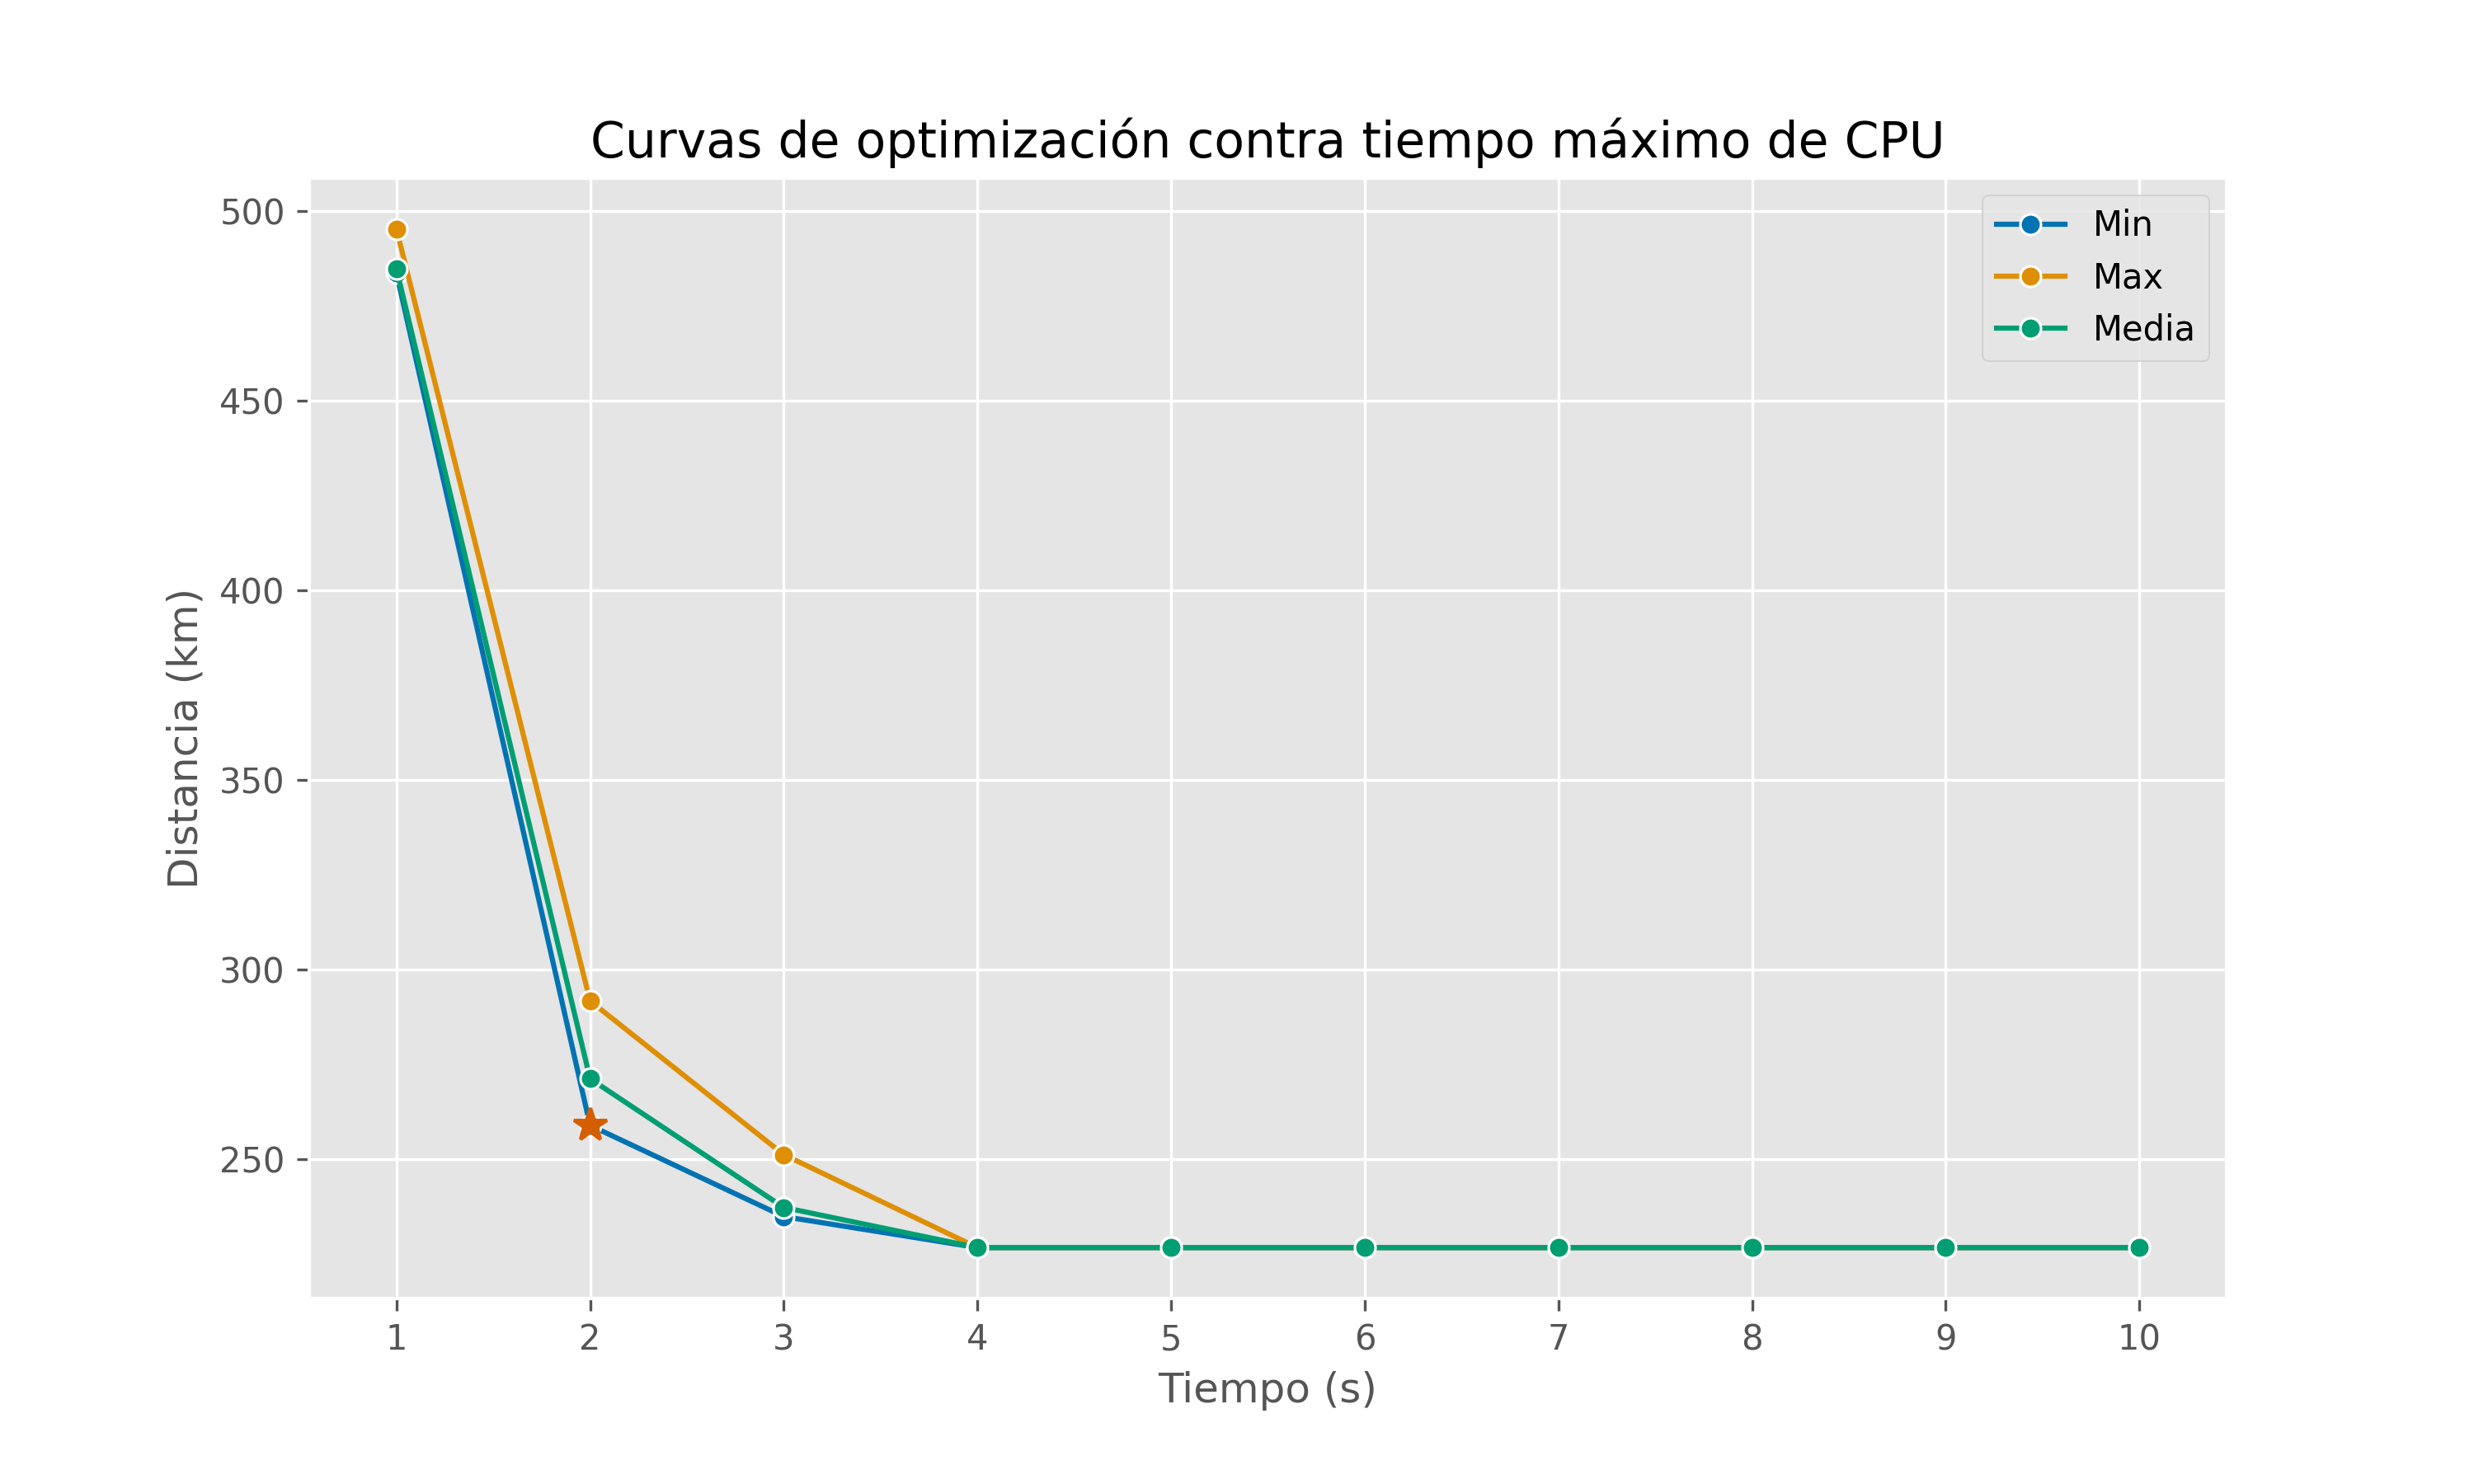
\includegraphics[scale=0.35]{../img/curvas-opt.png}
                \caption{Curva de optimización con diferentes tiempos máximos de cómputo}
                \label{fig:optim-curves}
            \end{figure}

            También hemos generado una curva para varianza den cada una de las observaciones:

            \begin{figure}[h!]
                \centering
                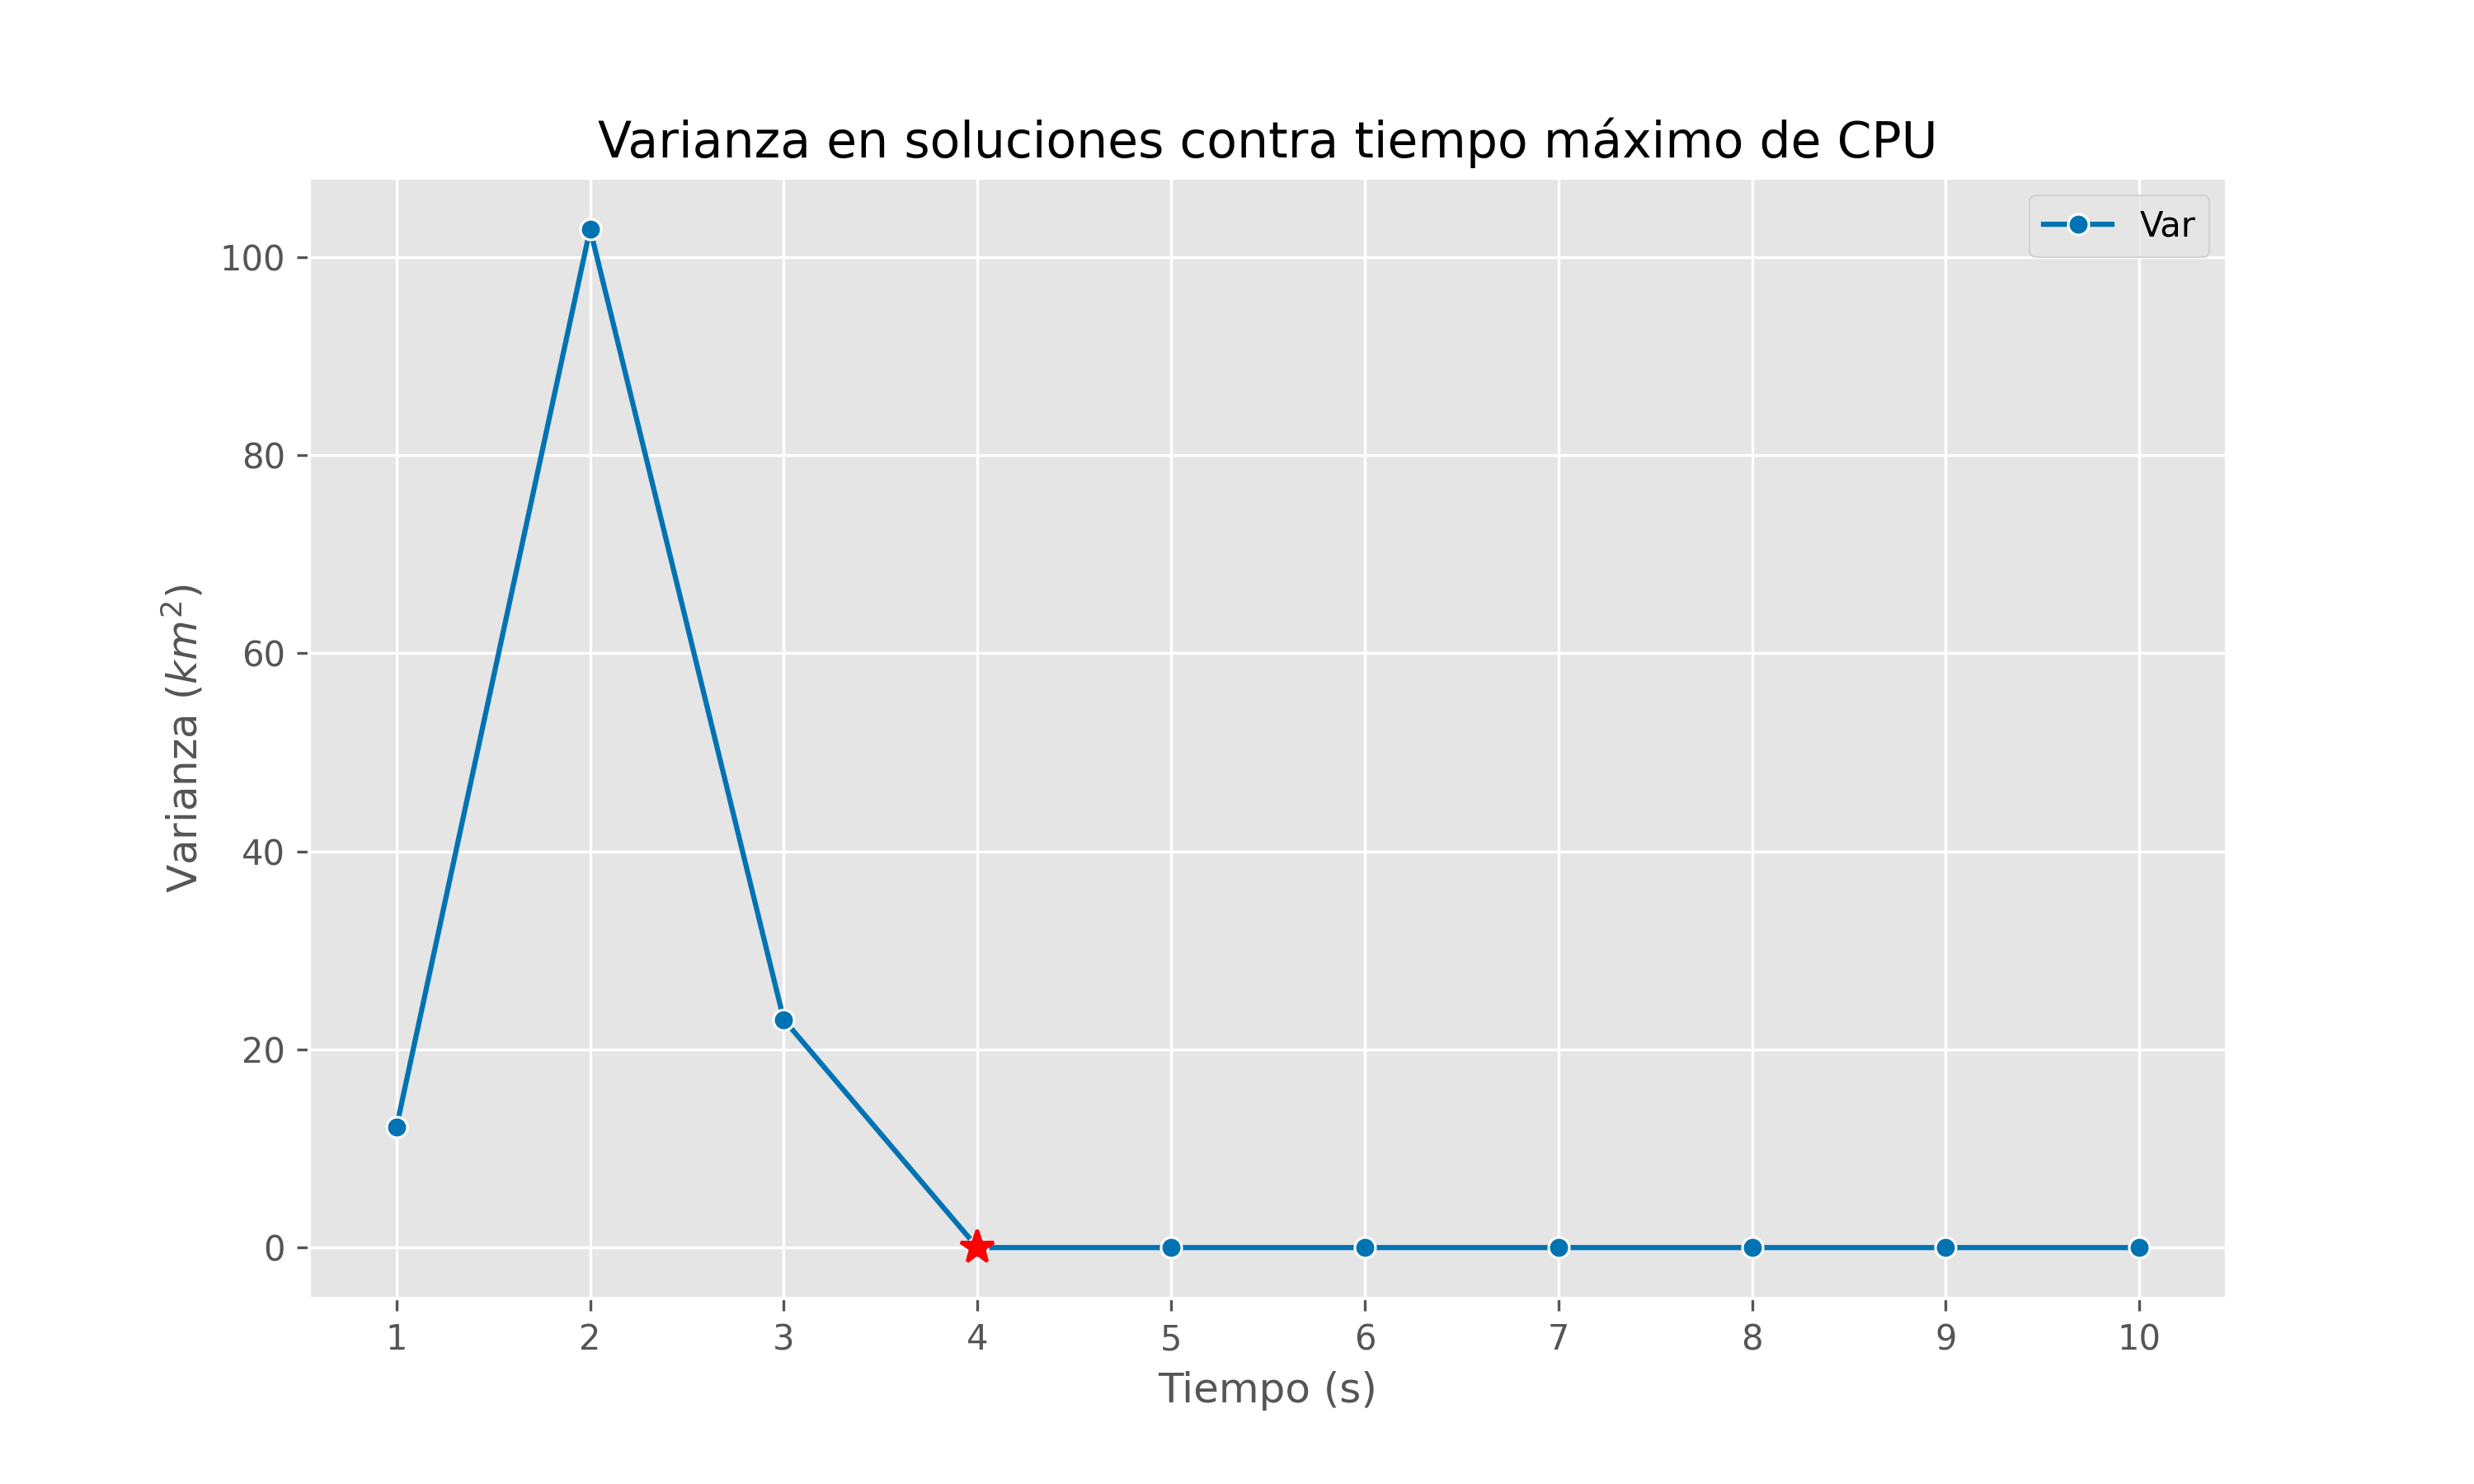
\includegraphics[scale=0.35]{../img/varianza-opt.png}
                \caption{Varianza de soluciones encontradas para diferentes tiempos máximos de cómputo}
                \label{fig:optim-var}
            \end{figure}

            De estas curvas después se utilizó la librería de \texttt{Python}, \texttt{kneed}. En ella se implementa el algoritmo propuesto por Satopaa en Finding a “Kneedle” in a Haystack: Detecting Knee Points in System Behavior \cite{satopaa2011finding}. En la figura \ref{fig:optim-curves} y en la figura \ref{fig:optim-var} se visualiza el punto encontrado.

            El punto de inflexión de la distancia mínima sugeriría que a partir de 2 segundos esta métrica no cambiará de forma drástica. Sin embargo, en la curva de la varianza este punto se localiza en 4 segundos. Con el fin de asegurar la mayor consistencia, sugerimos que para la generación de rutas se realicen 10 simulaciones con un tiempo máximo de cómputo por simulación de 4 segundos.

        \subsection{Resultados} \label{sec:results}

            Después de correr la aplicación con los parámetros definidos en \ref{sec:parameter-tuning}, se desplegará el navegador el conjunto de rutas de todos los vehículos, en la figura \ref{fig:generated-routes} podemos ver 2 de las rutas encontradas.
        
            \begin{figure}[H]
                \centering
                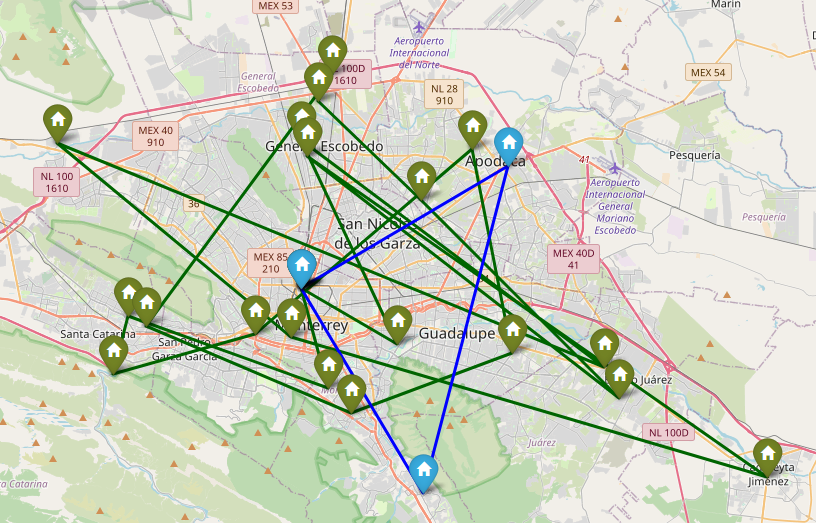
\includegraphics[scale=0.4]{../img/route-examples.png}
                \caption{Ejemplo de rutas generadas} 
                \label{fig:generated-routes}
            \end{figure}
            
            Como se puede apreciar en la tabla \ref{rutas}, para esta simulación, la aplicación encontró un conjunto de rutas que minimizan la distancia que recorren los camiones en total hasta 226.79 km. En esta solución el vehículo con la ruta más corta viaja 12.86 $km$ y el que tiene la ruta más larga viaja 42.21 $km$, se tiene una huella de carbono de 55 km de $CO_2$.
            
            \begin{table}[h!]
                \centering
                \scalebox{0.8}{
                \csvreader[tabular = ||c|c|c|c|c|c||,
                            table head = \hline N & Distancia $(km)$ & Carga $(m^{3})$ & Vol. muerto $(m^{3})$ & Gas $(l)$ & Huella $CO_2$ \\ \hline,
                            late after last line = \\ \hline,
                            ]{../data/processed/best_route.csv}{}%
                            {\csvcoli & \csvcolii & \csvcoliii & \csvcoliv & \csvcolv & \csvcolvi}}
                \caption{Rutas generadas por el programa}
                \label{rutas}
            \end{table}
            
    \section{Discusión de resultados} \label{sec:discusion}
        
        A pesar de que el producto que hemos desarrollado ya es funcional, hemos encontrado algunas áreas de oportunidad que de ser resueltas incrementarían aún más el valor de la aplicación.
        
        \subsection{Geo-codificación de los domicilios}
            
            Actualmente la aplicación hace uso de una librería de libre distribución llamada \texttt{Photon} para geo-codificar los domicilios disponibles en la base de datos; consideramos que la adquisición de una licencia comercial podría aumentar aún más el número de domicilios que son geo-codificados con éxito.
            
        \subsection{Cálculo de distancia entre 2 puntos}
            
            La aplicación utiliza como métrica de distancia la distancia geodésica, que está relativamente lejos de ser una aproximación rigurosa para determinar la distancia entre 2 puntos. Sugerimos también que se adquiera una licencia comercial que calcule esta distancia. Su uso le daría una mayor validez a los resultados que encontramos.
        
        \subsection{Variabilidad de resultados}

            El límite de tiempo máximo impuesto al proceso de optimización en nuestra aplicación está ligado al número máximo de cálculos por segundo del equipo usado; en caso de que nuestro sistema sea implementado en un ordenador con un mayor poder de cómputo, el tiempo necesario para encontrar una solución óptima se vería reducido.

        \subsection{Tiempo de cómputo}

            El proceso de la aplicación podría ser condensado a 4 etapas, limpieza de datos, geo-codificación de domicilios y cálculo de matriz de distancias, optimización y despliegue de resultados. Se han realizado 10 simulaciones de las que se calculó el tiempo promedio de ejecución, dichos resultados se presentan en la tabla \ref{table:execution-times}:

            \begin{table}[h!]
                \centering
                \begin{tabular}{ ||c|c|| }
                    \hline
                    Proceso & Tiempo (s) \\
                    \hline
                    Limpieza de datos & 7.7 \\
                    \hline
                    Geo-codificación y matriz de distancias & 777 \\
                    \hline
                    Optimización & 42.3 \\
                    \hline
                    Despliegue de rutas & 1.18 \\
                    \hline
                \end{tabular}
                \caption{Tiempos de cómputo de cada proceso}
                \label{table:execution-times}
            \end{table}

            El tiempo total de ejecución es de 13 minutos con 48 segundos, tiempo del cual el proceso de geo-codificación representa el 93.8\% de la operación completa. Pensamos que el uso de un software más avanzado podría reducir drásticamente este tiempo de ejecución. Sin embargo, hay que destacar que el tiempo de geo-codificación puede ser mitigado con una base de datos en la que se lleve un registro de los domicilios de los clientes en conjunto con sus coordenadas asociadas.
        
    \section{ODS} \label{sec:ods}
    
        Igual que encontrar la ruta más eficiente para la empresa, buscamos tener un impacto social por esta razón reconocemos la importancia que tiene que la innovación trascienda los objetivos personales, así como a los objetivos colectivos. Por eso mismo, tenemos la intención de tener un impacto positivo en los Objetivos de Desarrollo Sostenible propuestos por la ONU \cite{united-nations-2015}. 
        
        Una de las ODS implementadas en el proyecto es el objetivo número 9,  Industria, Innovación e Infraestructura, ya que los valores de esta ODS se alinean perfectamente con los de nuestro proyecto. Este objetivo tiene como enfoque la construcción de infraestructuras resilientes en forma de rutas adaptables que se basan en las necesidades, la industrialización sostenible en forma de la minimización de kilómetros recorridos y por lo tanto energía ocupada, e innovación de un sistema ya existente. 
        
        Otro de los objetivos en los que impactamos positivamente es el número 11, Ciudades y Comunidades Sustentables, ya que reconocemos que el mundo está cada vez más urbanizado, y la sostenibilidad no se puede quedar atrás. El e-commerce está cada vez más presente en las vidas de la gente, y al minimizar los efectos negativos de esta industria es el mejor paso que podemos tomar para un futuro verde. 

    \section{Recursos utilizados} \label{sec:resources}
        
        La implementación propuesta fue corrida en una máquina virtual de sistema operativo Ubuntu 20.04.3 LTS (Focal Fossa). El equipo disponía de un procesador Intel(R) Core(TM) i5-1035G1 CPU @ 1.00GHz, tenía disponible 8 GB de RAM.

        Especificaciones sobre los paquetes usados pueden ser encontrados en la documentación de nuestro repositorio \ref{code:repo}.

    \section{Conclusiones} \label{sec:conclusions}
        
        El ruteo de vehículos sigue siendo uno de los retos más relevantes para la Investigación de Operaciones, el diseño de algoritmos eficientes que logren encontrar rutas de entrega óptimas con cantidades cada vez más grandes de puntos de entrega es un imperativo para cualquier departamento de logística.
        
        Dado el gran número de puntos de entrega y de la enorme cantidad de posibles rutas a explorar, el uso de algoritmos heurísticos que logren encontrar rutas sub-óptimas es una alternativa a considerar para cualquier empresa; el que estos métodos puedan encontrar soluciones buenas en tiempos razonables hace que sean mucho más sencillos de implementar en producción.
        
        El proceso de determinar cuál es el mejor sub-conjunto de rutas tendrá tanto repercusiones económicas para la empresa como ecológicas para el ambiente, el proyecto que hemos desarrollado busca reducir la mayor cantidad de distancia recorrida posible por parte de las rutas, lo cual trae consigo una disminución del gasto realizado en el transporte de sus productos, mientras que se reducen en general las emisiones de carbono de sus vehículos.
        
    \appendices
    
    \section{Código fuente}\label{code:repo}
    
        El código generado puede ser consultado \href{https://github.com/JuanEcheagaray75/capacitated-vrp}{aquí}
    
    \bibliographystyle{IEEEtran}
    \bibliography{references.bib}

\end{document}
